\documentclass{article}



\usepackage{arxiv}

\usepackage[utf8]{inputenc} % allow utf-8 input
\usepackage[T1]{fontenc}    % use 8-bit T1 fonts
\usepackage{hyperref}       % hyperlinks
\usepackage{url}            % simple URL typesetting
\usepackage{booktabs}       % professional-quality tables
\usepackage{amsfonts}       % blackboard math symbols
\usepackage{nicefrac}       % compact symbols for 1/2, etc.
\usepackage{microtype}      % microtypography
\usepackage{graphicx}
\usepackage{doi}
\usepackage{array}
\usepackage{array}
\usepackage{censor}
\usepackage{paralist}
\usepackage{xcolor}
\usepackage{colortbl}
\usepackage{footmisc}
\usepackage{tikz}
\usepackage{pgfplots}
\usepackage{booktabs}
\usepackage{multirow}
\usepackage{placeins}
\usepackage{amsmath}
\usepackage{subcaption}
\usepackage{comment}
\usepackage{float}


\title{Hope vs. Hate: Understanding  User Interactions with LGBTQ+ News Content in Mainstream US News Media through the Lens of Hope Speech}

%\date{September 9, 1985}	% Here you can change the date presented in the paper title
%\date{} 					% Or removing it

\author{ \hspace{1mm}Jonathan Pofcher \\
        Rochester Institute of Technology
        \\
        \texttt{jep7453@rit.edu} \\
	%% examples of more authors
       \And
        Christopher M. Homan
        \\ 
        Rochester Institute of Technology 
        \\ 
        \texttt{cmhvcs@rit.edu }
        \And
        Randall Sell
        \\
        Drexel University 
        \\
        \texttt{randy@drexel.edu }
        \And
        Ashiqur R. KhudaBukhsh \thanks{Ashiqur R. KhudaBukhsh is the corresponding author}
        \\ 
        Rochester Institute of Technology
        \\   
        \texttt{axkvse@rit.edu}
	%% \AND
	%% Coauthor \\
	%% Affiliation \\
	%% Address \\
	%% \texttt{email} \\
	%% \And
	%% Coauthor \\
	%% Affiliation \\
	%% Address \\
	%% \texttt{email} \\
	%% \And
	%% Coauthor \\
	%% Affiliation \\
	%% Address \\
	%% \texttt{email} \\
}

% Uncomment to remove the date
%\date{}

% Uncomment to override  the `A preprint' in the header
\renewcommand{\headeright}{}
\renewcommand{\undertitle}{}
\renewcommand{\shorttitle}{Hope vs. Hate}

%%% Add PDF metadata to help others organize their library
%%% Once the PDF is generated, you can check the metadata with
%%% $ pdfinfo template.pdf

\begin{document}
\maketitle

\begin{abstract}
This paper makes three contributions. 
First, via a substantial corpus of 1,419,047 comments posted on 3,161 YouTube news videos of major US cable news outlets, we analyze how users engage with LGBTQ+ news content. Our analyses focus both on positive and negative content. In particular, we construct a fine-grained \textit{hope speech} classifier that detects positive (\textit{hope speech}), negative, neutral, and irrelevant content. Second, in consultation with a public health expert specializing on LGBTQ+ health, we conduct an annotation study with a balanced and diverse political representation and release a dataset of 3,750 instances with fine-grained labels and detailed annotator demographic information. Finally, beyond providing a vital resource for the LGBTQ+ community, our annotation study and subsequent in-the-wild assessments reveal (1) strong association between rater political beliefs and how they rate content relevant to a marginalized community; (2) models trained on individual political beliefs exhibit considerable in-the-wild disagreement; and (3) zero-shot large language models (LLMs) align more with liberal raters.  
\end{abstract}


\section{Introduction}


From crowdsourced storymapping projects sharing stories of love, loss, and a sense of belonging~\cite{kirby2021queering} to safe, anonymous spaces to seek resources~\cite{mcinroy2019lgbtq+} and dating platforms~\cite{blackwell2015seeing} -- the internet and modern technologies play a positive role in health and well-being of the LGBTQ+ community in various ways. However, cyberbullying~\cite{abreu2018cyberbullying}, exposure to dehumanization through news media~\cite{Mendelsohn_2020}, and more recently, worrisome homophobic biases in large language models~\cite{IJCAI2024RabbitHole} - are some of the modern technology perils the community grapples with. 

\textit{How do mainstream US cable news outlets cover the LGBTQ+ community and how do users interact with such news content?} Via a substantial corpus of more than 130 million YouTube comments on more than 300K YouTube news videos uploaded on three major US cable news outlets, this paper investigates how LGBTQ+ discussions are situated in mainstream US political discourse. While prior literature has analyzed LGBTQ+ discourse in print media through the lens of a dehumanization framework~\cite{Mendelsohn_2020}, such analyses consulted a single source of news (The New York Times) and did not consider reader responses to LGBTQ+ news. In this work, we consider three major US cable news networks representing diverse political views (Fox News, CNN, and MSNBC) with a key goal to understand how users interact and engage with LGBTQ+ news content. In doing so, we not only focus on identifying negative discussions about the LGBTQ+ community, one of our key contributions is operationalizing the detection of positive, \textit{hope speech} championing the disadvantaged minority in the broader spirit of counter-speech literature~\cite{benesch2014countering,mathew2019thou,palakodety2019hope,chakravarthi-2020-hopeedi,DBLP:conf/naacl/HenglePSBA024}. 



\begin{table*}[t]
\centering
\small
\begin{tabular}{|p{0.85\textwidth}|p{0.1\textwidth}|}
\hline
\textbf{YouTube Comment} & \textbf{Label} \\
\hline
\rowcolor{red!15}
\textit{This is why we have 500+ million guns in america. 
We need to start using them.
If a man walked in my daughters bathroom, that would be his last day on earth.
People arent gonna keep tolerating this. 
Theres about to be rainbow street justice youre gonna start seeing.  When comes to my, or anyones kids, and i frankly dont care what your laws. Never did in the first place, but when it comes to my kid……ill wake up and chose violence EVERY time. You christians can worry about the jesus nonsense. Keep “turning the other cheek” and here tf we are. The right republicans and media love their witty banter BUT WHAT EXACTLY TF DO YOU ACTUALLY DO?!!!!!!!!!!!!! NOTHING.} & Negative \\
\hline
\rowcolor{red!15}
 \textit{Hey if using the term f\censor{a}g is hate speech, then I stand guilty as charged. I hate what they stand for and I hate the corruption they're bringing into society, and I especially hate that they are preying on the minds of children  in an attempt to make them believe that their sick, perverted lifestyle is normal.  I don't use the term gay because they have hijacked the term to ease the reality of who they are. Gay used to mean " a happy person"  which is far from what these people are.}
 & Negative \\
\hline
\rowcolor{blue!15}
\textit{LISTEN PEOPLE: EVEN IF YOU DONT SUPPORT IT, YOU CAN RESPECT US AT LEAST. ALL WE WANT IS BASIC HUMAN DECENCY. LITERALLY JUST THAT. me and my girlfriend got spat at on a bus once, and then called homophobic slurs. we just want respect, being gay doesn't change the fact that I'm a human. JUST BE NICE TO EVERYONE AND STOP CARING SO MUCH ABT OTHER PEOPLE AND THEIR BUSINESS.}
& Positive \\
\hline
\rowcolor{blue!15}
\textit{Reading these comments are making me cry. I'm 13 and my Dad is transgender. 99\% of Doctors accept it. Why are you one to argue with Science? Please, if you are a bigot, don't reply to this comment. It will make me cry. I love my Dad, and you ignorant people who don't accept science won't change that. Please don't reply to this comment unless you have something nice to say.}& Positive \\
\hline
\end{tabular}
\caption{Illustrative examples of positive and negative YouTube comments identified by our classifier in the wild}
\label{tab:youtube-comments}
\end{table*}

%In recent years, the prevalence of hate speech in online communities, in addition to real world harm caused by it, has increased significantly. This is an even more substantial issue in spaces relevant to those who are a part of marginalized groups, such as the LGBTQ+. Traditional approaches of dealing with hate speech, such as censorship and  punitive measures, have shown limited efficacy and potential backlash, prompting a shift towards alternative strategies. While counter-speech strategies offer value, their reactive nature necessitates the presence of harmful content to be effective. In contrast, our research enables a proactive approach: the promotion of hope speech, which aims to cultivate digital environments characterized by empathy, acceptance, and constructive dialogue.


While hate speech detection and mitigation strategies have been extensively researched (see, e.g., \cite{fortuna}), relatively little attention has gone into the opposite: \textit{hope speech}. Defined as comments and posts that inspire optimism and diffuse hostility in online spaces~\cite{palakodety2019hope,chakravarthi-2020-hopeedi}, hope speech is crucial for groups who face a disproportionate amount of hate speech.  In the current US cultural climate, where issues of race, gender, and sexuality are at the forefront of the so-called “culture war”~\cite{hartman2019war}, there is a need for tools that can detect both positive and negative content as listed in Table~\ref{tab:youtube-comments} and increase understanding of relevant online conversations. 

\noindent\textbf{Contributions.} Our contributions are as follows.

\noindent\textcolor{blue}{(1)}. In consultation with a health expert specializing in LGBTQ+ health for more than two decades, we curate a novel dataset of 3,750 instances with fine-grained labels: \textit{neutral}, \textit{irrelevant}, \textit{positive} (hope speech), and \textit{negative}\footnote{Will be made publicly available upon acceptance.}. Each instance is labeled by three annotators (one Republican, one Democrat, and one independent) ensuring diverse and balanced political perspectives in the annotation process. Several raters self-identified as being part of the LGBTQ+ community.\\
\textcolor{blue}{(2)}. We analyze the association between rater political beliefs and how they rate content relevant to LGBTQ+ community.\\
\textcolor{blue}{(3)} We analyze the alignment of large language models with political beliefs in connection with LGBTQ+ content and investigate how rater biases perpetuate into fine-tuned models.\\  
\textcolor{blue}{(4)}. We provide novel insights into audience engagement patterns and sentiment dynamics
surrounding LGBTQ+ content, enhancing our
understanding of LGBTQ+ discussions within mainstream US political discourse. To our knowledge, no such study exists at our scale. 

\begin{figure*}[htb]
    \centering
    \includegraphics[width=0.9\textwidth]{latex/Images/Comment_Annotation_Diagram.pdf}
    \caption{Corpus annotation pipeline}
    \label{fig:dataset}
\end{figure*}

\section{Related Work}

Our work is closely related with the \textit{hope speech} literature~\cite{palakodety2019hope,palakodety2020voice,chakravarthi-2020-hopeedi} and the broader literature of counter speech~\cite{benesch2014countering,mathew2019thou,DBLP:conf/naacl/HenglePSBA024,DBLP:conf/ijcai/SahaSKM022,DBLP:conf/acl/GuptaDGB0A23}. Our work contributes to this literature through our unique focus on LGBTQ+ discourse in mainstream US politics and our investigation on how rater subjectivity and political leanings. 

Political polarization in the US is widely studied across multiple disciplines in rich and diverse settings that include congressional voting patterns on policy issues~\cite{poole1984polarization}, mate selection~\cite{huber2017political}, allocation of scholarship funds~\cite{iyengar2015fear}, and annotating offensive content~\cite{sap-etal-2022-annotators,Vicarious}. While how political leanings might associate with the task of rating negative content has been studied both in the context of US politics~\cite{sap-etal-2022-annotators,Vicarious} and on hot button issues such as reproductive rights, gun control/rights~\cite{Vicarious}, and US infrastructure~\cite{InfrastructureOmbudsman}, our work demonstrates that political identities of the raters may influence how they perceive positive content for the LGBTQ+ community. Our study thus contributes to the broader literature of annotator subjectivity~\cite{pavlick2019inherent,sap2019risk, al2020identifying, larimore2021reconsidering, sap-etal-2022-annotators, goyal2022your, pei-jurgens-2023-annotator, Vicarious, homan2024intersectionality, prabhakaran2024grasp}. 

Our annotation study design is grounded in prior literature~\cite{sap-etal-2022-annotators,Vicarious} and draws from~\cite{Vicarious} in seeking diverse and balanced political perspectives including from the independents. Our work also touches upon political bias in LLMs as we observe that zero-shot classification of LGBTQ+ content of several models are more aligned with liberal raters~\cite{feng-etal-2023-pretraining,bang-etal-2024-measuring}. To tackle class imbalance, we construct an ensemble active learning pipeline much akin to~\cite{palakodety2020voice} leveraging well-known active learning strategies (e.g., certainty sampling~\cite{sindhwani2009uncertainty} and margin sampling~\cite{scheffer2001active}).  

%Developing machine learning and NLP models for hope speech detection offers potential insights into online discourse patterns and the varied reception of supportive content across different internet demographics. Within this under-explored field, two areas stand out as particularly promising for further investigation: hope speech directed towards the LGBTQ+ community and the application of state-of-the-art Large Language Models (LLMs) for its detection and analysis.

%\par Our research offers three significant contributions to the emerging field of hope speech detection:

%\begin{enumerate}
%    \item We extend the concept of hope speech specifically for the LGBTQ+ community, constructing an annotated dataset of supportive comments, in the context of US politics.
    
%    \item We provide novel insights into audience engagement patterns and sentiment dynamics surrounding LGBTQ+ content, enhancing our understanding of digital discourse in these spaces.

    
%    \item We analyze the impact of political views on the creation and recognition of LGBTQ+ supportive content, providing insights into the intersection of politics and online discourse.
%\end{enumerate}

%\par This study represents the first application of large language models (LLMs) to examine LGBTQ+ hope speech at this scale and specificity. By creating and analyzing a novel dataset from comments on FOX, CNN, and MSNBC YouTube videos, we aim to advance hope speech detection techniques and explore the distribution of positive LGBTQ+ discourse among different audiences. The results of our model demonstrate the significant impact that both negative and positive comments can have in online spaces. As shown in Table \ref{tab:youtube-comments}, negative comments can often contain explicit threats, derogatory language, and harmful stereotypes that can create a hostile environment for LGBTQ+ individuals. In contrast, positive comments express support, empathy, and calls for respect, potentially creating a more welcoming atmosphere. For instance, one supportive comment emphasizes the desire for "basic human decency" and respect.  Our work not only seeks to improve technical models but also contributes to the broader goal of fostering a more inclusive digital landscape for marginalized communities.


\section{Dataset and Annotation Study Design}




Figure~\ref{fig:dataset} presents a schematic diagram of our data collection process described in details next. 

\subsection{YouTube News Videos}

We consider a dataset of 333,032 YouTube videos uploaded between 04/10/2008 to 08/31/2024 by the official YouTube channels of three major US cable news networks: Fox News, CNN, and MSNBC. First introduced in~\cite{KhudaBukhshPolarization}, this dataset represents a reliable snapshot of US political discourse encompassing diverse political perspectives over a substantial period of time. This dataset has found prior use in studying  (1) election misinformation~\cite{Capitol}; (2) health misinformation~\cite{yoo2023auditingrobustifyingcovid19misinformation}; and (3) annotation subjectivity~\cite{Vicarious}.   

% We chose YouTube because it allowed us to gather a large set of political discourse and discussion through the comments section. Looking at these three mainstream news networks also gave us a diverse set of political affiliations and ideological leanings based on the target audience of each channel. Beyond studying political polarization, this dataset has been used to study (1) election misinformation \cite{inproceedings}; (2) health misinformation \cite{yoo2023auditingrobustifyingcovid19misinformation}; (3) content moderation subjectivity \cite{weerasooriya}.

%The process through which we took these videos and their comments and created an annotated corpus for LGBTQ+ Hope Speech is diagrammed in Figure 1. and will be explained in more detail below. 


\subsection{Identifying LGBTQ+ Relevant Videos}

%The first step of our process was filtering out the videos from these channels that were not related to LGBTQ+ topics. LGBTQ+ Hope Speech is already a very rare class among our results and using comments from every possible video would make the identification and collection of sufficient examples difficult and very expensive. 

%In order to do this filtering we utilized a ChatGPT pipeline. While we first looked at simple keyword filtering, we found that it did not perform as well as expected; it missed a significant amount of videos with more subtle references to LGBTQ+ in the title and did not collect a desired quantity of videos. Initial tests of ChatGPT proved promising, so we moved forward with that approach. 



In contrast to prior literature predating highly capable LLMs, which used keyword filtering to prune large datasets for relevance (see, e.g.,~\cite{o2010tweets,demszky-etal-2019-analyzing,halterman-etal-2021-corpus}), we conduct our filtering using LLMs using a two-step process. First, for each video, we pass the video title and description to \texttt{GPT-4o mini} prompting it to classify the video as specifcially relevant to the LGBTQ+ community or not  (Appendix contains prompt details in \S~\ref{sec:Prompt}). This step prunes our initial set of 333,032 videos down to 5,435 videos. Next, for each of these 5,435 videos, we use the same prompt and pass the video title and description to \texttt{GPT-4o}. We use this two-step process because although the \texttt{GPT-4o} model performed better and ended up with slightly fewer false positives, it was considerably more expensive to run it on all 333,032 videos. Overall, through this two-step process, we obtain 3,161 relevant videos (denoted by $\mathcal{V}_\textit{LGBTQ+}$). A manual inspection of 300 random videos (100 from each news outlet) reveals only 2 false positives indicating that $\mathcal{V}_\textit{LGBTQ+}$ is highly relevant for LGBTQ+ issues.  

%Our pipeline consisted of two steps. First we passed the video title and description to the "GPT-4o mini" model with the prompt displayed in Table 1. Then we would take all of the positives found from that, and pass them to the more powerful "GPT-4o" to filter out any false positives that may be found. We used this two-step process because, although the full "GPT-4o" model performed better and ended up with slightly fewer false positives, it was significantly more expensive and more time consuming and we could not run it on all 313,000 videos. The "GPT-4o mini" model allowed us to filter the amount of videos down to a few thousand before proceeding and we ended up with 3,161 videos related to LGBTQ+ content from the three YouTube channels.
%There was a total of 1,420,399 comments left on these videos. By taking a sample of 300 comments, 100 from each channel, we found only two false positives, showing us the robustness of this pipeline. Table 2. shows a few interesting examples of true positives and false positives found in our results.
\begin{table*}[t]
\scriptsize
\setlength{\tabcolsep}{2pt}
\renewcommand{\arraystretch}{1.2}
\begin{tabular}{|>{\raggedright\arraybackslash}p{0.22\textwidth}|>{\raggedright\arraybackslash}p{0.28\textwidth}|>{\raggedright\arraybackslash}p{0.39\textwidth}|>{\raggedright\arraybackslash}p{0.11\textwidth}|}
\hline
\textbf{Video title} & \textbf{Video description} & \textbf{\texttt{GPT-4o} explanation} & \textbf{Classification} \\
\hline
\rowcolor{gray!15}
Attacks On Abortion Rights Already Forcing Women To Dangerous 'Back Alley' Alternatives & 
Dr. Bhavik Kumar, medical director of primary and trans care at Planned Parenthood Gulf Coast, talks with Rachel Maddow about the desperation and hardship the Texas abortion ban is causing people seeking abortion services to which they have a right, and explains that the longer term restrictions on reproductive rights are already forcing people seeking abortions into dangerous circumstances. & 
The video features Dr. Bhavik Kumar, who is the medical director of primary and trans care at Planned Parenthood Gulf Coast. Although the main topic of the video is about the attacks on abortion rights in Texas, the mention of "trans care" in Dr. Kumar's professional role suggests that the topic might be relevant to transgender people, who are a part of the LGBTQ+ community. However, since the description doesn't explicitly state this, it's not a certainty, but a possibility. & 
False Positive \\
\hline
\rowcolor{white!15}
Montel Williams slams North Carolina's 'bathroom bill' &
Activist talks problematic articles within the controversial legislation on 'The Kelly File' &
The video seems to be relevant to the LGBTQ+ community based on the reference to North Carolina's 'bathroom bill,' a controversial legislation that affected the rights of transgender people, which makes it pertinent to their interests and concerns. Montel Williams being noted as an activist, alongside mentioning 'problematic articles' in the bill, suggests a discussion about these LGBTQ+ issues. &
True Positive \\
\hline
\end{tabular}
\caption{Videos identified as LGBTQ+ relevant by our \texttt{GPT-4} pipeline}
\label{tab:GPTExplanation}
\end{table*}
\par

Table~\ref{tab:GPTExplanation} shows an example true positive and a false positive found in our results. The first shows a case in which the video ended up not being LGBTQ+ relevant, except for the fact that the person featured is a director of trans care, but the video does not focus on that fact. It is interesting that \texttt{GPT-4o} actually acknowledges this in its explanation, however did end up still flagging it as relevant. The second is an example that identifies the \textit{bathroom bill} as relevant to LGBTQ+ issues. 
%\texttt{GPT-4o} is able to correctly identify that this is referring to a bill which would affect the bathroom's transgender individuals could use. 

\subsection{Constructing $\mathcal{D}_\textit{hope}$}

For each video in $\mathcal{V}_\textit{LGBTQ+}$, we collect user comments using publicly available YouTube API yielding 1,419,047 comments. From these comments, we construct $\mathcal{D}_\textit{hope}$, a dataset with fine-grained labels of posts supportive of the LGBTQ+ community. In consultation with the health expert specializing on LGBTQ+ health research for more than two decades, we identify four broad categories: \textit{positive} (\textit{hope speech}); \textit{negative}; \textit{irrelevant}; and \textit{neutral}. Detailed annotation guidelines are present in the Appendix (\S ~\ref{sec:guidelines}). 

In brief, this process consists of three steps:
\begin{compactenum}
\item We first construct a seed set of 1,950 instances using a collaborative human-LLM annotation framework. This seed set is annotated by crowd-sourced annotators for the aforementioned four categories  (details are described in \S~\ref{sec:human-LLM}). This step yields $\mathcal{D}_\textit{seed}$ consisting of 649 positives, 150 negatives, 87 neutrals, and 660 irrelevants and a validation set $\mathcal{D}_\textit{eval}$ of 250 instances set aside for all performance evaluation. 
\item Next, we conduct minority class certain sampling~\cite{sindhwani2009uncertainty} of additional 900 instances to address class imbalance (details are described in \S~\ref{sec:ActiveLearning}). This step yields $\mathcal{D}_\textit{certainty}$ consisting of 680 positives, 682 negatives, 227 neutrals, and 764 irrelevants. 
\item Finally, we conduct margin sampling~\cite{scheffer2001active}, a well-known variant of uncertainty sampling (described in \S~\ref{sec:ActiveLearning}). This step yields $\mathcal{D}_\textit{margin}$ consisting of 824 positives, 947 negatives, 314 neutrals, and 1,020 irrelevants.   
\end{compactenum}



% It was given a train/test split of 70/30 for 6 epochs, making use of QLoRa in order to train such a large language model. 


\subsubsection{Annotating $\mathcal{D}_\textit{hope}$}\label{sec:CrowdsourcedAnnotation}

We use Prolific, a well-known crowd-sourcing platform, to gather and pay raters and hosted the survey on Qualtrics. Our study follows a similar annotation design as \cite{Vicarious} in the sense that we consider raters evenly distributed across three political leanings (Republican, Democrat, and Independent). We split our corpus into a set of 65 batches, each containing an equal amount of comments from each channel and containing/not containing hope speech. Each batch is labeled by three annotators (one Republican, one Democrat, and one Independent). Since we do not want to expose raters to objectionable content for a sustained period, following standard practices, our batch size is limited to 30 instances. We compensate each rater \$0.10 for each example. This yields a compensation of \$3 for each batch. We observe a median task completion time of 11:53 minutes, implying an hourly wage estimate of \$15.16, more than the minimum wage. This annotation compensation is grounded in prior literature \cite{leonardelli-etal-2021-agreeing,bai-etal-2021-pre,Vicarious}. We also left an unstructured text feedback input for each of the workers. No one complained about the compensation. Many subjects thanked us for providing an interesting and thought-provoking task, while some responded to the survey with homophobia, which might lead to interesting follow-on research (Appendix contains sample responses). Our study was reviewed by our Institutional Review Board and was deemed as exempt.

Our study asked the raters to annotate each comment with one of the following labels (in regards to sentiment towards the LGBTQ+ community) (1) Positive, (2) Negative, (3) Neutral, or (4) Irrelevant. In pilot test surveys, we tried asking raters to pick one of only two labels, Positive or Not Positive. This appeared to make the task more challenging as due to less nuance and granularity in the annotation process, shown by lower agreement between annotators. The choice to switch to four labels (advised by the health expert) also benefited us by introducing more detailed information for analysis and training of models. %After completion of the survey we had our dataset of 1950 comments from LGBTQ+-related videos, each given a label by three annotators of different political affiliations. This process was repeated twice more for sampling.

 On our final annotated dataset, the Fleiss' $\kappa$ for all four labels is 0.431 and for just two labels (\textit{HopeSpeech} (positive) and \textit{not-HopeSpeech} (neutral, negative, and irrelevant)) is 0.485. This shows relatively moderate agreement between all annotators. For a challenging task like this, involving analysis of sentiment towards a specific community, which can be affected by personal beliefs and values, we observe considerably high agreement. Interestingly, the agreement remains relatively stable when expanding from two to four labels, indicating consistent annotator judgment across different levels of classification detail.


\section{Classification Results}
%A main contribution of our research is progress towards a machine learning classifier to identify hope or hate speech directed towards the LGBTQ+ community. 

We consider \texttt{Mistral} (Mistral-7B-Instruct-v0.3)~\cite{jiang2023mistral} and \texttt{Llama 3} (Llama-3-8B-Instruct)~\cite{dubey2024llama}, two well-known open LLMs for fine-tuning. For each LLM, we construct four models - three individual political affiliation specific models, and one aggregate model trained on majority label.      
We determine the aggregate label by taking a majority vote, a standard approach to resolving annotator disagreement (see, e.g.,~\cite{davidson2017automated,wiegand2019detection}). Any comments that received three separate labels are not used in the aggregate data, accounting for 11.3\% of instances, however we used these instances for political affiliation specific models. 

%A majority of these were introduced during the sampling process, where annotators were recieving more difficult comments. The LLMs that we tested were Llama 3 and Mistral v0.3, both with 7B parameters. From our starting corpus of 1950 crowd-labelled comments, we separated a random set of 250 to use as an unseen validation set for all experiments.

Table~\ref{tab:model-comparison2} summarizes our models' performance on $\mathcal{D}_\textit{eval}$. We consider both zero-shot and fine-tuned models (Appendix contains prompt details in \S~\ref{sec:Prompt}). For fine-tuning, we use a sequence classification head. We split the training data, after removing the validation set, into an 80/20 test/train split and train for 5 epochs, considering the best model as the one with the highest Macro-F1. Initially, we only consider fine-tuning a model on aggregate labels, but once we determined the highest-performing model, we fine-tuned additional ones specific to each political affiliation (Table~\ref{tab:political-agreement-finetuned} describes the noise audit results of these models). We use standard machine learning performance metrics such as accuracy, macro-averaged precision, recall, and F1, as well as the class-specific F1 scores. We find (1) the fine-tuned models considerably outperform zero-shot models; (2) the models' performance improvement gradually across different stages of the active learning pipeline; and (3) the best-performing model is \texttt{Llama 3} trained on $\mathcal{D}_\textit{margin}$.
 



%\subsection{Zero-Shot Classification}
%To do an initial test of the LLM models, we performed Zero-Shot classification by asking it to generate text based on a prompt including each comment. The prompt used for four label can be seen in Figure \ref{fig:4label_prompt}. By limiting the amount of tokens generated and filtering the responses, we were able to get an answer corresponding to a label for every instance. We calculated accuracy and metrics for the results with the ground truth as consensus label, as well as for each political affiliation. 

%\subsection{Fine-tuned Classification}


 %While the zero-shot classifications performed surprisingly well for a multi-class problem, however were significantly improved upon with the initial fine-tuning. 


\begin{table*}[t]
\centering
\footnotesize
\setlength{\tabcolsep}{4pt}
\begin{tabular*}{\textwidth}{@{\extracolsep{\fill}}l|cccc|cccc@{}}
\hline
& \multicolumn{4}{c|}{\texttt{Llama}~\cite{dubey2024llama}} & \multicolumn{4}{c}{\texttt{Mistral}~\cite{jiang2023mistral}} \\
\textbf{Metric} & $\mathcal{M}(.)$ & $\mathcal{M}(\mathcal{D}_\textit{seed})$ & $\mathcal{M}(\mathcal{D}_\textit{certainty})$ & $\mathcal{M}(\mathcal{D}_\textit{margin})$ & $\mathcal{M}(.)$ & $\mathcal{M}(\mathcal{D}_\textit{seed})$ & $\mathcal{M}(\mathcal{D}_\textit{certainty})$ & $\mathcal{M}(\mathcal{D}_\textit{margin})$  \\
\hline
Accuracy & 0.5520 & 0.8304±0.01 & \textbf{0.8376±0.01} & 0.8224±0.02 & 0.6640 & 0.8024±0.03 & 0.7640±0.08 & 0.7840±0.09 \\
\hline
\multicolumn{9}{l}{\textbf{Macro-averaged metrics:}} \\
Precision & 0.5468 & 0.7286±0.03 & \textbf{0.7378±0.03} & 0.7127±0.04 & 0.5654 & 0.6549±0.12 & 0.6549±0.07 & 0.6510±0.12 \\
Recall & 0.5547 & 0.6289±0.01 & 0.6688±0.02 & \textbf{0.6740±0.01} & 0.5488 & 0.5845±0.07 & 0.6453±0.06 & 0.6276±0.10 \\
F1 Score & 0.4768 & 0.6507±0.02 & 0.6838±0.02 & \textbf{0.6850±0.02} & 0.5375 & 0.5923±0.08 & 0.6376±0.07 & 0.6258±0.11 \\
\hline
\multicolumn{9}{l}{\textbf{Class-specific F1 scores:}} \\
Positive & 0.6845 & 0.8571±0.01 & \textbf{0.8595±0.01} & 0.8422±0.02 & 0.8312 & 0.8345±0.03 & 0.7898±0.06 & 0.7986±0.09 \\
Negative & 0.3009 & 0.5801±0.02 & \textbf{0.6344±0.06} & 0.6130±0.05 & 0.4545 & 0.4269±0.19 & 0.5620±0.11 & 0.5487±0.20 \\
Neutral & 0.2553 & 0.2373±0.09 & 0.3004±0.09 & \textbf{0.3574±0.09} & 0.1765 & 0.1971±0.11 & 0.3037±0.08 & 0.2381±0.13 \\
Irrelevant & 0.6667 & 0.9281±0.01 & \textbf{0.9409±0.01} & 0.9276±0.01 & 0.6879 & 0.9108±0.02 & 0.8949±0.08 & 0.9178±0.04 \\
\hline
\end{tabular*}
\caption{\small{Comparison of \texttt{Llama} and \texttt{Mistral} model results on aggregate labels over five independent training runs. Values are shown as mean±standard deviation where applicable. $\mathcal{M}(.)$ denotes the zero-shot performance. $\mathcal{M}(\mathcal{D})$ denotes model performance when fine-tuned on $\mathcal{D}$. Best results for each metric across all models and settings are shown in bold.}}
\label{tab:model-comparison2}
\end{table*}

\section{Substantive Findings}

We break down our findings into three separate subsections. 

\subsection{User Engagement with $\mathcal{V}_\textit{LGBTQ+}$ Videos}

Recall that, $\mathcal{V}_\textit{LGBTQ+}$ represents a set of 3,161 news videos relevant to LGBTQ+ issues. In order to compare and contrast user engagement with these videos, we construct a control set (denoted by $\mathcal{V}_\textit{control}$). Each video $\textit{v}$ in $\mathcal{V}_\textit{LGBTQ+}$ is matched with a video that is (1) not relevant to LGBTQ+ issues; (2) is uploaded by the same news outlet; (3) has roughly same video duration as $\textit{v}$; and (4) has the publishing time closest to $\textit{v}$.   

Let for a given video $v$, $v_\textit{likes}$, $v_\textit{dislikes}$, $v_\textit{views}$, and $v_\textit{comments}$ denote the total number of likes, dislikes, views and comments on $v$, respectively. 
Following~\cite{Lopez-youtubers,Entube,braun2017enhanced,KhudaBukhshPolarization}, we calculate engagement rate and dislike ratio for a given video as follows. 

\textit{engagementRate(v)} = $\frac{v_\textit{likes} + v_\textit{dislikes} + v_\textit{comments}}{v_\textit{views}}$ \\

\textit{dislikeRate(v)} = $\frac{v_\textit{dislikes}}{v_\textit{likes} + v_\textit{dislikes}}$ 

Table \ref{tab:dislike-engagement-rates} compares the engagement rate and dislike rates of videos in $\mathcal{V}_\textit{LGBTQ+}$ and $\mathcal{V}_\textit{control}$. YouTube stopped allowing  users to access dislikes starting in 2021, so our dislike rate data only includes videos up until that point\footnote{sourced from \url{https://github.com/Suji04/YouTube-Dislike-Dataset}}. We observe that LGBTQ+ videos consistently received higher dislike rates across all three channels compared to non-LGBTQ+ content. This difference is most pronounced for FOX News and CNN, with smaller but still noticeable differences for MSNBC. Overall engagement rates for LGBTQ+ videos are generally lower than for non-LGBTQ+ content, though the magnitude of this difference varied by news outlet. FOX News showed the largest decrease in engagement for LGBTQ+ content, while CNN and MSNBC exhibited differences small enough to likely be insignificant.

The higher dislike ratios and lower engagement rate for LGBTQ+ content across all news outlets, regardless of perceived political leaning, point to a persistent societal resistance to LGBTQ+ topics. Although, this resistance is shown to be more pronounced for the most conservative channel, FOX News. %It is worth noting again that our data collection controls for upload date and video duration, indicating that these observed differences are likely related to content type rather than external temporal factors or video length disparities.
 

\begin{table}[h]
\centering
\footnotesize
\begin{tabular}{@{}llcccc@{}}
\hline
\textbf{Outlet} & \textbf{Type} & \multicolumn{2}{c}{\textbf{Dislike Rate}} & \multicolumn{2}{c}{\textbf{Engagement Rate}} \\
 & & \textbf{Mean} & \textbf{Med.} & \textbf{Mean} & \textbf{Med.} \\
\hline
\multirow{2}{*}{MSNBC} & $\mathcal{V}_\textit{control}$ & 22.7\% & 13.5\% & 2.69\% & 2.47\% \\
 & $\mathcal{V}_\textit{LGBTQ+}$ & 24.1\% & 18.8\% & 2.60\% & 2.30\% \\
\hline
\multirow{2}{*}{FOX} & $\mathcal{V}_\textit{control}$ & 18.7\% & 10.6\% & 3.40\% & 3.29\% \\
 & $\mathcal{V}_\textit{LGBTQ+}$ & 29.7\% & 20.8\% & 2.63\% & 2.52\% \\
\hline
\multirow{2}{*}{CNN} & $\mathcal{V}_\textit{control}$ & 27.3\% & 21.2\% & 1.69\% & 1.31\% \\
 & $\mathcal{V}_\textit{LGBTQ+}$ & 35.5\% & 32.4\% & 1.66\% & 1.30\% \\
\hline
\end{tabular}
\caption{\small{Dislike and Engagement Rates by outlet and video type.}}
\label{tab:dislike-engagement-rates}
\end{table}

%Understanding how politics interacts with minority rights in NLP technologies will remain a pressing challenge.


 


\subsection{Annotation Study Findings}

Prior literature reports association of raters' political leanings with the way they annotate toxic content \cite{sap-etal-2022-annotators,Vicarious}. We observe similar results when looking at the agreement between annotators for our task. In Table \ref{tab:political-agreement}, we observe partisan differences in annotation. The agreement between Democrats and Independents is  higher than the agreement between either group and Republicans. This suggests that even given the same comment text and annotation guidelines, Republicans and Democrats or Independents may have different conclusions as to what is positive or negative speech towards the LGBTQ+ community. Even if we collapse the fine-grained labels into \textit{HopeSpeech} and \textit{not-HopeSpeech}, the qualitative findings on political disagreement remain unchanged (see, Appendix).

\par Our survey also include a question asking the raters if they considered themselves a member of the LGBTQ+ (raters can opt out of answering this question), allowing us to analyze if differences in sexual orientation would impact annotation. Out of 375 study participants, 98 identified themselves as being LGBTQ+. The Cohen's $\kappa$ agreement between LGBTQ+ and non-LGBTQ+ annotators is 0.449. This agreement fits nicely between the low value found when comparing Republicans to others, and the high value found comparing Independents and Democrats. It is quite close to the overall Fleiss' $\kappa$ of 0.431. This is particularly interesting and indicates that even for a topic highly relevant to gender and sexual orientation, rater disagreement is impacted more by political leanings than sexual orientation. Once again, if we collapse the labels into \textit{HopeSpeech} and \textit{not-HopeSpeech}, the qualitative findings on disagreement remain unchanged (see, Appendix).

\begin{table}[t]
\centering
\scriptsize
\setlength{\extrarowheight}{2pt}
\begin{tabular}{cc|c|c|c|}
  & \multicolumn{1}{c}{} & \multicolumn{1}{c}{\textit{Dem}}  & \multicolumn{1}{c}{\textit{Rep}}  & \multicolumn{1}{c}{\textit{Ind}} \\\cline{3-5}
            & \textit{Dem} &\cellcolor{blue!25} - & 0.408  & 0.477
 \\ \cline{3-5}
 & \textit{Rep} & \textcolor{black}{0.408} &\cellcolor{blue!25} - & \textcolor{black}{0.396}
 \\\cline{3-5}
            & \textit{Ind} & \textcolor{black}{0.477} & \textcolor{black}{0.396 }  &\cellcolor{blue!25} - \\\cline{3-5}
\end{tabular}
%\vspace{0.2cm}
\caption{\small{Human rater agreement across political affiliations. A cell $\langle i,j\rangle$ presents the Cohen's $\kappa$ agreement between raters with political affiliation $i$ and $j$. \textit{Dem}, \textit{Rep}, and \textit{Ind} denote Democrat, Republican, and Independent, respectively.}}
\label{tab:political-agreement}
\end{table}

%\begin{table}[t]
%\centering
%\scriptsize
%\setlength{\extrarowheight}{2pt}
%\begin{tabular}{cc|c|}
%  & \multicolumn{1}{c}{} & \multicolumn{1}{c}{\textit{Non-LGBT}} \\\cline{3-3}
%            & \textit{LGBT} & 
% \\\cline{3-3}
%\end{tabular}
%\caption{{Four-Label LGBTQ+ Agreement}}
%\label{tab:lgbt-agreement}
%\end{table}

In addition to our main model fine-tuned on the aggregate labels, we also fine-tune models specifically on the labels of each political affiliation (denoted by $\mathcal{M}_\textit{rep}$, $\mathcal{M}_\textit{dem}$, and $\mathcal{M}_\textit{ind}$). Using each of these models, we classify a set of 50k unseen comments from each channel. Following~\cite{kahneman2021noise,Vicarious}, we conduct a noise audit of these models as shown in Table \ref{tab:political-agreement-finetuned}. While we observe the in-the-wild agreement across models is higher than the agreement across human raters with different political beliefs, the impact of the political affiliations still shone through. Once again, Democrats and Independents share higher agreement with each other, while they both have lower agreement with Republicans to a similar degree. This demonstrates that the human biases due to political affiliation in labelled data can perpetuate to fine-tuned models. Tables~\ref{tab:political-comments},~\ref{tab:political-commentsHumans} present illustrative examples showing how trans-exclusionary stance of human Republican raters may get perpetuated to fine-tuned LLM $\mathcal{M}_\textit{rep}$ affecting marginalized voices. 

%The biggest difference is that the agreements overall are quite a bit higher. This is likely because, while fine-tuned, it is the same base model underneath, while every human annotator is a different person with their own beliefs and biases. Despite this

\begin{table}[t]
\centering
\scriptsize
\setlength{\extrarowheight}{2pt}
\begin{tabular}{cc|c|c|c|}
  & \multicolumn{1}{c}{} & \multicolumn{1}{c}{$\mathcal{M}_\textit{dem}$}  & \multicolumn{1}{c}{$\mathcal{M}_\textit{rep}$}  & \multicolumn{1}{c}{$\mathcal{M}_\textit{ind}$} \\\cline{3-5}
            & $\mathcal{M}_\textit{dem}$ &\cellcolor{blue!25} - & 0.572  & 0.670
 \\ \cline{3-5}
 & $\mathcal{M}_\textit{rep}$ & \textcolor{black}{0.572} &\cellcolor{blue!25} - & \textcolor{black}{0.573}
 \\\cline{3-5}
            & $\mathcal{M}_\textit{ind}$ & \textcolor{black}{0.670} & \textcolor{black}{0.573}  &\cellcolor{blue!25} - \\\cline{3-5}
\end{tabular}
%\vspace{0.2cm}
\caption{{In-the-wild Cohen’s $\kappa$ agreement of models trained on data annotated by raters with same political affiliation.}}
\label{tab:political-agreement-finetuned}
\end{table}


\begin{table}
\centering
\scriptsize
\begin{tabular}{|p{0.6\linewidth}|p{0.10\linewidth}|p{0.10\linewidth}|}
\hline
\textbf{Comment} & $\mathcal{M}_\textit{rep}$ & $\mathcal{M}_\textit{dem} $, $\mathcal{M}_\textit{ind}$ \\
\hline
\textit{Since when was having a phobia such a bad thing? You wouldnt say this about some scared of heights of or spiders… there freaks amd theres nothing to be ashamed of when having a transphobia} &
Positive &
Negative \\
\hline
\textit{damn! first time I've seen Tucker actually lose. I love you Tucker, but the military transgender ban is BS. it's not a huge expense. Like Sean Patrick said in the end before Tucker rage quits "They're earning those benefits by putting their life on the line for America and have done more for this country than you (Tucker) and I ever will". Hormones arent expensive. 10ml testosterone costs \$40 and it lasts them 6 months.} &
Negative &
Positive \\
\hline
\end{tabular}
\caption{\small{Illustrative examples were $\mathcal{M}_\textit{rep}$ does not agree with $\mathcal{M}_\textit{dem}$ and $\mathcal{M}_\textit{ind}$. }}
\label{tab:political-comments}
\end{table}

\begin{table}[htb]
\centering
\scriptsize
\begin{tabular}{|p{0.6\linewidth}|p{0.10\linewidth}|p{0.10\linewidth}|}
\hline
\textbf{Comment} & \textit{Rep} & \textit{Dem} \& \textit{Ind} \\
\hline
\textit{Good Job America - Keep it UP- GO WOKE GO BROKE - Transheuser-Busch deserves IT} &
Positive &
Negative \\
\hline
\textit{Thank you so much for sharing. Your story highlights how messed up the treatment is for Trans people.} &
Negative &
Positive \\
\hline
\end{tabular}
\caption{\small{Disagreements in labels across human raters on Prolific. \textit{Rep}, \textit{Dem}, and \textit{Ind} denote Republican, Democrat, and Independent, respectively.}}
\label{tab:political-commentsHumans}
\end{table}


We also calculate the performance metrics of zero-shot classification against the annotations of each political affiliation (see, Table \ref{tab:political-affiliation-comparison}). The results show similar performance with Democrat and Independent labels, but each metrics was lower for the Republican labels. This was present across the three different models we tested; \texttt{GPT-4o-mini}, \texttt{Llama}, and \texttt{Mistral}. This suggests that the biases present in these models may align closer with the biases found in our human Independent and Democrat annotators, than those of a Republican.

\begin{table}
\centering
\setlength{\tabcolsep}{3pt}
\footnotesize
\begin{tabular*}{\textwidth}{@{\extracolsep{\fill}}l|ccc|ccc|ccc@{}}
\hline
\multirow{2}{*}{\textbf{Metric}} & \multicolumn{3}{c|}{\textbf{GPT-4o-mini}} & \multicolumn{3}{c|}{\textbf{Meta-Llama-3-8B}} & \multicolumn{3}{c}{\textbf{Mistral-7B-v0.3}} \\
\cline{2-10}
 & \textbf{Dem.} & \textbf{Rep.} & \textbf{Ind.} & \textbf{Dem.} & \textbf{Rep.} & \textbf{Ind.} & \textbf{Dem.} & \textbf{Rep.} & \textbf{Ind.} \\
\hline
Accuracy & \textbf{0.5963} & 0.5520 & 0.5864 & 0.5143 & 0.4809 & 0.5091 & 0.5354 & 0.4954 & 0.5260 \\
\hline
\multicolumn{10}{l}{\textbf{Macro-averaged metrics:}} \\
Precision & \textbf{0.6146} & 0.5664 & 0.6057 & 0.4534 & 0.4101 & 0.4484 & 0.4316 & 0.4019 & 0.4236 \\
Recall & \textbf{0.5839} & 0.5391 & 0.5717 & 0.3803 & 0.3497 & 0.3736 & 0.4178 & 0.3849 & 0.4061 \\
F1 Score & \textbf{0.5749} & 0.5320 & 0.5636 & 0.3716 & 0.3401 & 0.3653 & 0.4080 & 0.3790 & 0.3990 \\
\hline
\multicolumn{10}{l}{\textbf{Class-specific F1 scores:}} \\
Positive & \textbf{0.7236} & 0.6464 & 0.7113 & 0.5801 & 0.5102 & 0.5609 & 0.6586 & 0.5884 & 0.6469 \\
Negative & \textbf{0.6509} & 0.6171 & 0.6330 & 0.5846 & 0.5670 & 0.5781 & 0.6103 & 0.5571 & 0.5886 \\
Neutral & \textbf{0.3406} & 0.3233 & 0.3264 & 0.2096 & 0.1718 & 0.1943 & 0.2604 & 0.2537 & 0.2453 \\
Irrelevant & \textbf{0.5843} & 0.5412 & 0.5840 & 0.4840 & 0.4513 & 0.4930 & 0.5108 & 0.4957 & 0.5141 \\
\hline
\end{tabular*}
\caption{\small{Zero-shot model results across political affiliation specific labels evaluated on the full human annotated corpus of 3,750 comments.}}
\label{tab:political-affiliation-comparison}
\end{table}

\subsection{In-the-wild Hope Speech Analyses}

In order to look at the hope and hate speech make-up of LGBTQ+ discussion in-the-wild, we consider our best-performing model and classify 50k randomly sampled, unseen comments from each news outlet. The results, as shown in Figure \ref{fig:label-breakdown-with-ci}, reveal distinct patterns. Notably, FOX News stands out with the highest proportion of negative comments (24.15\%) and the lowest proportion of positive comments (2.3\%) among the three outlets. This aligns with the outlet's reputation for conservative viewpoints. In contrast, CNN shows a more balanced distribution, with the highest percentage of positive comments (7.66\%) and a negative comment rate (17.2\%) closer to the overall average. MSNBC, interestingly, has a much lower proportion of positive comments than CNN (4.55\%) and the lowest proportion of negative comments (9.36\%).
  %To ensure the robustness of our findings and estimate the precision of our results, we employed a bootstrap sampling technique, resampling our dataset 50 times with replacement. 
 \par 
\par To get a better understanding of the sentiment of these comments sections we introduce the Positivity Ratio. 
\vspace{-0.2cm}
\[
\text{Positivity Ratio} = \scriptsize\frac{\#\text{Positive Comments}}{\#\text{Positive Comments} + \#\text{Negative Comments}}
\]

\begin{figure}
\centering
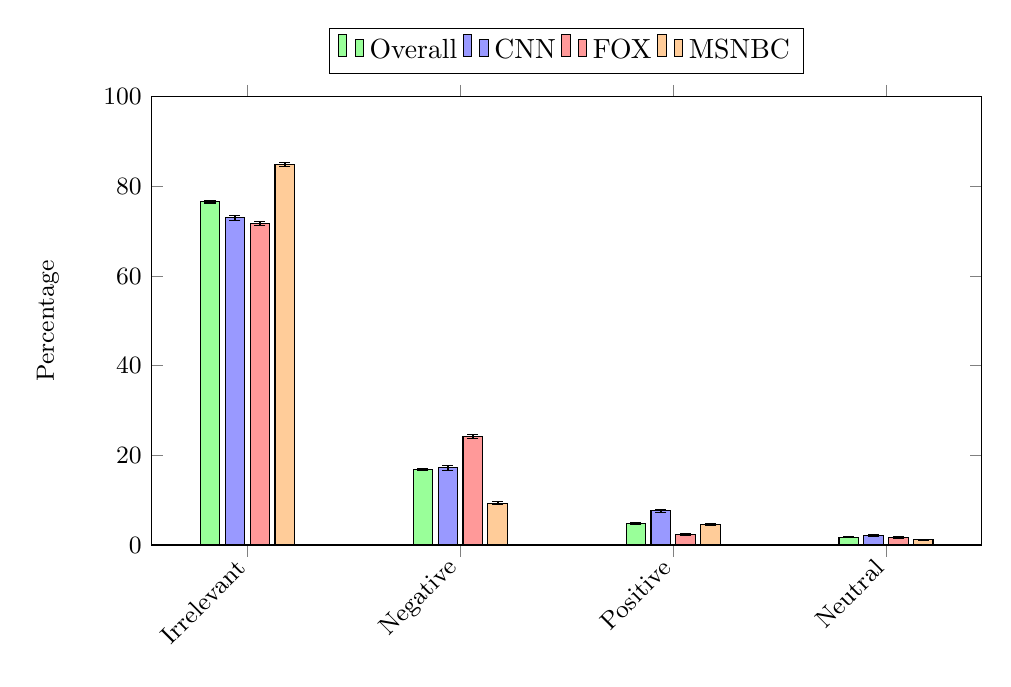
\begin{tikzpicture}
\begin{axis}[
    width=\columnwidth,
    height=0.6\columnwidth,
    ybar,
    bar width=7pt,
    enlarge x limits={0.15},
    legend style={at={(0.5,1.05)}, anchor=south, legend columns=-1},
    ylabel={Percentage},
    symbolic x coords={Irrelevant, Negative, Positive, Neutral},
    xtick=data,
    x tick label style={rotate=45,anchor=east},
    ymin=0,
    ymax=100,
    scaled y ticks = false,
    ylabel near ticks,
    title style={font=\large},
    label style={font=\small},
    tick label style={font=\small},
    y label style={at={(axis description cs:-0.1,.5)}, anchor=south},
    error bars/y dir=both,
    error bars/y explicit,
    error bars/error bar style={line width=0.75pt, color=black},
]
\legend{Overall, CNN, FOX, MSNBC}
\addplot[fill=green!40, error bars/.cd, y dir=both, y explicit] 
    coordinates {
        (Irrelevant, 76.53) +- (0.25, 0.25)
        (Negative, 16.90) +- (0.25, 0.25)
        (Positive, 4.84) +- (0.15, 0.15)
        (Neutral, 1.73) +- (0.1, 0.1)
    };
\addplot[fill=blue!40, error bars/.cd, y dir=both, y explicit] 
    coordinates {
        (Irrelevant, 72.96) +- (0.6, 0.6)
        (Negative, 17.20) +- (0.5, 0.5)
        (Positive, 7.66) +- (0.35, 0.35)
        (Neutral, 2.19) +- (0.2, 0.2)
    };
\addplot[fill=red!40, error bars/.cd, y dir=both, y explicit] 
    coordinates {
        (Irrelevant, 71.78) +- (0.45, 0.45)
        (Negative, 24.15) +- (0.45, 0.45)
        (Positive, 2.30) +- (0.2, 0.2)
        (Neutral, 1.77) +- (0.2, 0.2)
    };
\addplot[fill=orange!40, error bars/.cd, y dir=both, y explicit] 
    coordinates {
        (Irrelevant, 84.87) +- (0.45, 0.45)
        (Negative, 9.36) +- (0.4, 0.4)
        (Positive, 4.55) +- (0.2, 0.2)
        (Neutral, 1.22) +- (0.1, 0.1)
    };
\end{axis}
\end{tikzpicture}
\caption{Label breakdown by news outlets with 95\% confidence intervals. 50k comments from each news outlet found in-the-wild were classified by our best performing model.}
\label{fig:label-breakdown-with-ci}
\end{figure}

\begin{table*}
\centering
\footnotesize
\label{tab:label-breakdown-with-ci}
\begin{tabular}{lrrrr}
\hline
\textbf{Label} & \textbf{Overall} & \textbf{CNN} & \textbf{FOX} & \textbf{MSNBC} \\
\hline
Irrelevant & 76.53\% ± 0.025\% & 72.96\% ± 0.06\% & 71.78\% ± 0.045\% & 84.87\% ± 0.045\% \\
Negative   & 16.90\% ± 0.025\% & 17.20\% ± 0.05\% & 24.15\% ± 0.045\% & 9.36\% ± 0.04\% \\
Positive   & 4.84\% ± 0.015\% & 7.66\% ± 0.035\% & 2.30\% ± 0.02\% & 4.55\% ± 0.02\% \\
Neutral    & 1.73\% ± 0.01\% & 2.19\% ± 0.02\% & 1.77\% ± 0.02\% & 1.22\% ± 0.01\% \\
\hline
Positive Ratio  & 22.25\% ± 0.065\% & 30.81\% ± 0.12\% & 8.70\% ± 0.07\% & 32.70\% ± 0.15\% \\
\hline
\end{tabular}
\caption{\small{Label breakdown and positivity rates by channel with 95\% confidence intervals. 50k comments from each channel
found in-the-wild were classified by our best performing model.}}
\end{table*}

This ratio focuses solely on comments expressing clear sentiment, excluding irrelevant and neutral comments to provide a more direct measure of sentiment polarity. By using this metric, we find that MSNBC has the highest positivity ratio at 32.7\%, followed closely by CNN at 30.81\%, both above the overall average of 22.25\%. In stark contrast, FOX News shows a significantly lower positivity ratio of 8.7\%. These findings further emphasize the divergence in audience sentiment across channels, with MSNBC and CNN fostering more balanced or slightly positive discussions around LGBTQ+ content, while FOX News comments lean heavily towards negative sentiment.
\par
Perhaps the most important results come from looking at the trends as a whole. For every channel, there were more negative comments than positive ones. This consistent imbalance, favoring negative sentiment across all channels, suggests a broader societal tendency towards critical or oppositional engagement with LGBTQ+ topics in online spaces. It implies that, regardless of the platform, viewers are more inclined to express disapproval or criticism than support or affirmation when commenting on LGBTQ+-related content. Another noteworthy trend is the uniformly low percentage of neutral comments across all channels, ranging from 1.22\% to 2.22\%. This scarcity of neutral perspectives, coupled with the positive-negative imbalance, points to a highly polarized discourse surrounding LGBTQ+ issues. It suggests that those who engage in these comment sections tend to hold and express strong opinions, whether positive or negative, rather than maintaining a neutral stance.

\subsection{Error Analysis}


While our model performed well in identifying the rare class of LGBTQ+ hope speech in the wild, there were cases where the beliefs expressed in comments were too nuanced to be classified correctly. Table \ref{tab:error-examples} showcases two such examples. Both comments are generally supportive on a surface level. One is promoting human rights and social progress, the other is giving respect to female athletes. However, in context it is clear the support is not directed to the LGBTQ+. The first comment is equating the social progress of the LGBTQ+ community with bestiality, a common homophobic cliché. The second comment is specifically singling out "biological female athletes" to support, taking a clear stance on the issue of transgender people in sports.
\par Examples like these illustrate the challenges a task like this entails. Our model fails to fully understand the sarcasm or superficial support that less straight-forward comments may contain. Enhancing the model's ability to understand context and implicit meanings, possibly through the use of more advanced language models or improved tuning, is a worthy future research challenge. %Additionally, expanding the training dataset to include a wider range of nuanced examples could improve performance.

\begin{table}
\centering
\scriptsize
\begin{tabular}{|p{0.25\textwidth}|p{0.12\textwidth}|}
\hline
\textbf{YouTube Comment} & \textbf{Model Prediction} \\
\hline
\textit{Bestiality rights are human rights. Vote biden to continue social progress.} & Positive \\
\hline
\textit{Power and respect to her and all other biologically female athletes. STAY LOUD} & Positive \\
\hline
\end{tabular}
\caption{\small{Two example challenging comments our classifier mistakenly identified as Positive.}}
\label{tab:error-examples}
\end{table}




\begin{comment}
\begin{table*}[t]
\centering
\small
\begin{tabular}{|p{0.85\textwidth}|p{0.1\textwidth}|}
\hline
\textbf{YouTube Comment} & \textbf{Label} \\
\hline
Pride haha
Disgusting wicked act not pride.
You are Insane filthy people. & Negative \\
\hline
It's beyond time we perform a moral cleansing of society and rid ourselves of this perverted filth. & Negative \\
\hline
This is CRUEL for the "real biological" women. This is so wrong on every level. Just look at her, she's a BEAST. Too sad & Negative \\
\hline
These are not human beings. They have no feeling's at all. This is sick. & Negative \\
\hline
It's funny how straight people never have sexual identity issues. This "it" needs to be put out of "it's" misery, and "it's" parents should serve time in prison for letting "it" turn out this way. & Negative \\
\hline
\end{tabular}
\caption{Examples of "vermin metaphors" and dehumanization directed toward the LGBTQ+ community found in the wild}
\label{tab:vernin-examples}
\end{table*}
\end{comment}

\section{Conclusions}

In this paper, we present a comprehensive picture of LGBTQ+ discussions in mainstream US political discourse. Overseen by a health expert specializing in LGBTQ+ health for decades, we conduct a detailed annotation study  that reveals political biases of raters are associated with how they rate supportive content for the LGBTQ+ community. Our study shows that such biases may perpetuate into models affecting marginalized voices. Our in-the-wild assessment of LGBTQ+ discussions reveal that negative comments about the community considerably outweigh positive discourse indicating a technological gap to ensure safer spaces for marginalized communities.   

\section{Ethics Statement}

Our study was reviewed by our Institutional Review Board and was deemed as exempt. Our study is overseen by a health expert with decades of research on LGBTQ+ health. We investigate publicly available data collected using public APIs. 

We do not collect any PII (Personally Identifiable Information) about the raters and compensate them above the minimum wage. Since content moderation can be potentially gruesome and affect the
mental health of the raters~\cite{Guardian1}, we
maintain a small batch size (30 YouTube comments). 



While our goal
is to broaden our understanding of LGBTQ+ discussions in mainstream US political news and our content classifier can assist human moderators to identify supportive content for the LGBTQ+ community, any content
filtering system can be tweaked for malicious purposes. For instance, an inverse filter can be made
that filters out \textit{hopeSpeech} posts while filtering in \textit{not-hopeSpeech} 
ones.

Our substantive findings rely on fine-tuned large language models. Studies indicate that these models have a
wide range of biases that reflect the texts on which they were
originally trained, and which may percolate to downstream
tasks~\cite{bender2021dangers}. 

\section{Limitations}
While our study offers valuable insights into hope speech detection for LGBTQ+ topics in US political discourse, we recognize there are limitations that shape the scope and applicability of the findings.
\par
Our focus on YouTube comments for major news channels, while providing a rich dataset, is only a fraction of the online discource related to LGBTQ+. Platforms like Twitter, Reddit, and others have their own unique demographics, content, and user interactions. What we observed on YouTube may not be true for the rest of the internet, potentially limiting our generalizability across social media. 
\par Additionally, our study is grounded in US politics, where societal attitudes towards the LGBTQ+ have been affected by historical and legal context. However, LGBTQ+ rights and acceptance may vary dramatically across the world. In some countries, open support for LGBTQ+ rights might be more common and less contentious, while in others, it could be far more risky or even illegal to express such support. This global variation in LGBTQ+ rights and societal attitudes means that the patterns of hope speech and the very definition of what constitutes supportive language could differ significantly across cultural and national boundaries.

\par While our study did not specifically aim at participatory AI~\cite{harrington2019deconstructing,birhane2022power} as our key goal was to study the interplay of rater politics and how they perceive LGBTQ+ discussions, a considerable fraction of our raters self-reported as being part of the community. Future studies can solely focus on participatory AI involving more raters from the LGBTQ+ community and extend this research to vicarious interactions~\cite{Vicarious}. 

\par We also acknowledge that many challenges faced by individual groups within the LGBTQ+ community are unique. For instance, the trans community faces several additional challenges such as participation in competitive sports or access to gender reassignment treatment. Future studies solely focusing on the trans community will add further value to prior literature focusing on specific exclusionary behavior (see, e.g.,~\cite{lu-jurgens-2022-subtle}). 
\par In terms of political affiliations, while we attempted to capture the broad ideological difference present in the US, this may oversimplify their nuanced reality. Our categorization of political affiliations into the groups of "Democrat," "Republican," and "Independent" may not fully capture these nuances. In reality political views exist on a spectrum rather than in discrete categories. 
\par Finally, we acknowledge a lack of intersectionality analysis in our study. We have focused on LGBTQ+ identity and political affiliation, overlooking the possibility of intersection with factors such as race, ethnicity, age, or socioeconomic status. The interplay of these identities can have significant influence on how an individual perceives the LGBTQ+ community and speech surrounding it. Future work could be improved by capturing these complex intersection and identifying possible impact on LGBTQ+ and hope speech perception.





% Bibliography entries for the entire Anthology, followed by custom entries
%\bibliography{anthology,custom}
% Custom bibliography entries only
\clearpage
\bibliographystyle{unsrt}
\bibliography{hope}
\clearpage
\appendix

\section{Additional Related Work}
\subsection{Additional Literature on Counter Speech}

There exists a large body of research done into the automatic detection of hate-speech online. This is mainly relevant in the case of social media platforms such as Facebook or YouTube, where such hateful content can be very harmful to both user's online and in-person experiences, especially those belonging to marginalized or minority groups\cite{muller-karsten}. By identifying this hate-speech, either before or after it is posted, it can be censored or removed and the user's that posted such content can be warned or banned. In extreme cases, entire social media platforms can be taken down by those hosting them\cite{agarwal2022deplatforming}. More recent research has shown that censorship and suppression of offenders is not always the best way to deal with such situations. These approaches can often be unsuccessful in limiting the spread of hateful ideas and may even backfire, both in the context of social media and in society as a whole \cite{benesch2014countering}.
\par Counter-speech has been proposed as a method of mitigating the effects of and preventing hate-speech, without the need to limit free speech through censorship. Counter-speech is a somewhat vague term and current literature defines it in a multitude of ways and acknowledges that there are many different types and strategies of counter-speech that can be found online, each achieving varying levels of success in different communities. It was found that empathy-based approaches could cause posters of xenophobic hate-speech to delete their comments and be less likely to post similar content in the near feature \cite{hangartner2021}. However, it has also been shown that strategies such as utilizing a 'Positive Tone' or affiliating oneself with the marginalized group are often not effective and may even garner replies by other users stating that such comments will not change the opinions of the hate speakers \cite{mathew2019thou}. Another negative aspect of relying on counter-speech to moderate online communities is that it requires the existence of hate-speech to be employed. By most working definitions of counter-speech, it must be in reply to a hateful comment. This limits its effectiveness as it can only be used as a response and not proactively. 

\subsection{Additional Literature on Hope Speech}
Addressing the drawbacks of counter-speech and the complexities of censorship, the emerging field of hope speech research presents a promising approach. It focuses on promoting positive, inclusive dialogues, aiming to transform and de-escalate online communities into environments of support and mutual respect. The term hope speech started to be used a few years ago by authors looking for user posted content that aimed to diffuse conflict, for example, in the context of the tensions between Indian and Pakistan \cite{palakodety2019hope}. Before this, similar work had been done, but used other terms such as "help-speech" to refer to the positive discourse \cite{palakodety2020voice}. 
\par Since then, there have been multiple shared tasks in hope speech detection with over 50 teams presenting their findings \cite{chakravarthi-etal-2022-overview-shared} \cite{chakravarthi-muralidaran-2021-findings}. These shared tasks utilized datasets specifically created with hope-speech detection in mind, such as HopeEDI: a multi-lingual collection of almost 60,000 YouTube comments manually labeled as containing hope-speech or not \cite{chakravarthi-2020-hopeedi}. This dataset makes a point to contain hope speech directed at LGBTQ+ communities, among many other topics. Our study is different as it focuses directly on the LGBTQ+ community, but also views it through the lens of the US political divide. 
\par One related study that didn't explicitly focus on hope speech but provided valuable advancement to the field is the study of dehumanization. Dehumanization involves perceiving or treating people as less than human and often leads to extreme intergroup bias and hate speech. Mendelsohn, Tsvetkov, and Jurafsky developed a computational linguistic framework for analyzing dehumanizing language and applied it to discussions of LGBTQ people in the New York Times from 1986 to 2015 \cite{Mendelsohn_2020}. They found increasingly humanizing descriptions of LGBTQ people over time. Notably, different words with similar meanings, such as "gay" and "homosexual," had different levels of dehumanization, with "homosexual" being more associated with dehumanizing attitudes.
\par While much of the previous literature on hope speech detection mentions the LGBTQ+, as the task gravitates towards marginalized groups, there are gaps in research focusing directly on it. García‑Baena et al. created the dataset SpanishHopeEDI. It contains 1,650 annotated Spanish LGBTQ+-related tweets. A multitude of traditional machine-learning algorithms were tested on identifying hope-speech on them, leading to very impressive results \cite{garcia2023hope}. One related shared task similar to the previous ones was conducted focusing on this topic, however it was for hate-speech detection instead. For this, a dataset that specifically labelled LGBTQ+-related comments as homophobic or transphobic was used \cite{chakravarthi-etal-2022-overview}. %Currently, no equivalent dataset for LGBTQ+ hope speech in English exists.

\par Another important question for hope speech detection is understanding how subjective interpretations of language can impact the effectiveness of content moderation. A related study investigates the disagreement between human and machine moderators on what constitutes offensive speech in political discourse \cite{Vicarious}. This research highlights the challenges of subjectivity in moderation, revealing that both human and machine moderators often disagree on what is considered offensive, especially when political leanings are involved. These findings are relevant for hope speech detection as they underscore the need for nuanced understanding and handling of subjective content, ensuring that genuine hope speech is accurately identified amidst varying interpretations. In the same way that there can be disagreement on what is offensive, there can be disagreement on what is supportive or hopeful.


The recent introduction and consistent improvement of LLMs in the field of natural language processing has opened many new doors, and the task of hope speech detection is no different. However, at this point in time there has not been a lot of research into how effective LLMs are at hope-speech detection, never mind LGBTQ+ hope speech superficially. At the time of writing, only one paper has looked into this and attempted zero-shot ChatGPT prompting to label a Hope Speech dataset \cite{Ngo2023ZootopiAH}. They found that it resulted in poor performance for English texts, but was very successful for Spanish text. More work has been done surrounding LLM performance into hate-speech detection. The first extensive study into this found that prompting strategies had a significant impact on results \cite{guo2024investigationlargelanguagemodels}. They found using a Chain-of-Thought Reasoning Prompt had the highest results in all metrics and overall was effective in detecting hate-speech. 
%\par Not all related research on LLMs has focused on the detection of hate-speech or hope-speech, some has centered on how well LLMs can create these types of speech. One paper introduced what they called a "Toxicity Rabbit Hole" framework which could induce LLMs to produce toxic and offensive content despite the safety rails that are usually baked in \cite{dutta2024toxicityrabbitholenovel}. This demonstrates the double-sided nature of LLMs in their current state. While they may be used to detect and promote hope speech or identify and delete hate speech, it appears that currently it may be difficult to prevent them from creating hate speech as well.

\section{Prompts Used}\label{sec:Prompt}

\begin{figure}[H]
    \centering
    \includegraphics[width=\columnwidth]{latex/Images/LGBTQ_Prompt_1.pdf}
    \caption{Prompt for LGBTQ+ Video Classification}
    \label{fig:lgbtq_prompt}
\end{figure}

\begin{figure}[H]
    \centering
    \includegraphics[width=\columnwidth]{latex/Images/4Label_Prompt_1.pdf}
    \caption{Prompt used for  classification}
    \label{fig:4label_prompt}
\end{figure}

\section{Annotation Guidelines}
\label{sec:guidelines}
\par A comment is marked as \textbf{Hope Speech} if it meets any of the following criteria:
\begin{enumerate}
    \item Advocates for LGBTQ+ well-being, rights, or acceptance. 
    \textit{E.g.,} "How can we support LGBTQ+ youth in America?"
    
    \item Urges support for LGBTQ+ rights or anti-discrimination efforts. 
    \textit{E.g.,} "Politicians need to be against the Don't Say Gay Bill."
    
    \item Pushes for LGBTQ+ equal rights (marriage, anti-discrimination, gender recognition). 
    \textit{E.g.,} "Trans rights are human rights, and it's time for our laws to reflect that."
    
    \item Denounces anti-LGBTQ+ violence, discrimination, or hate speech. 
    \textit{E.g.,} "Homophobes need to be stopped."
    
    \item Shows sympathy for LGBTQ+ struggles and solidarity. 
    \textit{E.g.,} "I'm straight, but love is love!"
    
    \item Indirectly supportive and inclusive of LGBTQ+ community. 
    \textit{E.g.,} "Everyone deserves to love who they love, without fear or judgment."
\end{enumerate}

\par A comment is marked as \textbf{Non-Hope Speech} if it meets any of the following criteria:
\begin{enumerate}
    \item Expresses violent intent or supports discriminatory practices against LGBTQ+. 
    \textit{E.g.,} "If my kid has a gay teacher, they better watch out."
    
    \item Calls for actions/policies harmful to LGBTQ+ rights or well-being. 
    \textit{E.g.,} "Marriage should only be between a man and a woman."
    
    \item Diverts from LGBTQ+ issues to unrelated topics, diminishing their importance. 
    \textit{E.g.,} "I'm all for same-sex marriage, but should we worry about world hunger before this stuff?"
    
    \item Spreads misinformation or stereotypes about LGBTQ+ community. 
    \textit{E.g.,} "The alphabet mob is brainwashing our kids!"
    
    \item Demonstrates sarcastic or mocking support for LGBTQ+. 
    \textit{E.g.,} "Everyone should be able to identify as anything they want. I identify as an attack helicopter!"
    
    \item Unrelated to LGBTQ+ issues. 
    \textit{E.g.,} "Abortion is a sin!"
\end{enumerate}

\section{Two-Label Agreement}
\begin{table}[h]
\centering
\scriptsize
\setlength{\extrarowheight}{2pt}
\begin{tabular}{cc|c|c|c|}
  & \multicolumn{1}{c}{} & \multicolumn{1}{c}{\textit{Dem}}  & \multicolumn{1}{c}{\textit{Rep}}  & \multicolumn{1}{c}{\textit{Ind}} \\\cline{3-5}
            & \textit{Dem} &\cellcolor{blue!25} - & 0.447  & 0.556
 \\ \cline{3-5}
 & \textit{Rep} & \textcolor{black}{0.447} &\cellcolor{blue!25} - & \textcolor{black}{0.432}
 \\\cline{3-5}
            & \textit{Ind} & \textcolor{black}{0.556} & \textcolor{black}{0.432}  &\cellcolor{blue!25} - \\\cline{3-5}
\end{tabular}
\caption{Two-Label Political Affiliation Agreement (Human Annotators) Values are Fleiss' $\kappa$}
\label{tab:politicalAgreement}
\end{table}

\begin{table}[h]
\centering
\scriptsize
\setlength{\extrarowheight}{2pt}
\begin{tabular}{cc|c|}
  & \multicolumn{1}{c}{} & \multicolumn{1}{c}{\textit{Non-LGBT}} \\\cline{3-3}
            & \textit{LGBT} & 0.498
 \\\cline{3-3}
\end{tabular}
\caption{Two-Label LGBTQ+ Agreement (Human Annotators) Values are Fleiss' $\kappa$}
\label{tab:lgbtAgreement}
\end{table}

\section{Two-Label Classification Prompt}
\begin{figure}[h]
    \centering
    \includegraphics[width=\columnwidth]{latex/Images/2Label_Prompt_1.pdf}
    \caption{Prompt for 2-Label Classification}
    \label{fig:2label_prompt}
\end{figure}


\section{Curating $\mathcal{D}_\textit{hope}$}

\subsubsection{Initial Human and LLM Annotation}\label{sec:human-LLM}
Initially, one of the authors label a set of 1,500 comments (500 randomly sampled comments from three news outlets hosting $\mathcal{V}_\textit{LGBTQ+}$ videos) as being hope speech directed towards the LGBTQ+ community or not. See Appendix A for the guidelines used in this process. This step only identified 80 positives (5.33\%) i.e., LGBTQ+ hope speech suggesting that hope speech is a rare class. In order to curate a balanced dataset in a time- and cost-effective way, we turn to leveraging human-LLM collaborative annotation in the following way~\cite{wang2024human}. Using the initial labelled set of 1,500 comments, we fine-tune \texttt{Llama2-13B} (training details are in the Appendix). While this fine-tuned classifier was not highly accurate, it allowed us to identify hope speech more efficiently. We use this model to classify sets of 20,000 unseen comments from each channel. The same author as before went through the positives and verified any true positives until we obtain a total of 975 verified LBGTQ+ hope speech comments; 325 from each channel. These comments combined with a set of 975 random negatives labeled by the model, balanced for each channel, made up the 1,950 comment corpus that would be labelled by our crowd-sourced annotators as our seed set. 

We devote a separate subsection to describe our crowd-sourced annotation study design. In what follows, we outline our active learning steps to expand our seed set. 


\subsubsection{Active Learning}\label{sec:ActiveLearning}
We observe that our initial fine-tuned models performed considerably worse on the minority classes of \textit{Negative} and \textit{Neutral}, while they had relatively high performance on the \textit{Positive} and \textit{Irrelevant} classes. As a remedial measure, we employ two different active learning sampling strategies. 
\par The first was minority certainty sampling. Prior literature shows that this method can be useful for reducing class imbalance \cite{palakodety2020voice,attenberg-dual-supervision}. We consider our best-performing model at this point (a fine-tuned \texttt{Llama}) and have it classify an unseen set of 50k randomly sampled comments from each channel. We took the 150 comments of the highest certainty with labels \textit{Negative} and \textit{Neutral}, for each channel, totaling 900 instances.  We used the same crowd-sourced annotation design described in Section \ref{sec:CrowdsourcedAnnotation} to have these labelled. This allowed us to help close the gap in imbalance for these two labels. Our final dataset at this step was 2,850 instances. Looking at the distribution of comments with consensus among the annotators, we had 680 Positives, 682 Negatives, 227 Neutrals, and 764 Irrelevants. We found that this improved our model's performance, especially with the Neutral class, and were interested in seeing if continue sampling could improve it more.

\par Next we tried margin sampling. Using the now highest performing model, Llama trained on the certainty sampled data, we labelled 50,000 more comments from each channel. We looked at the margin of difference between the probability of the chosen label and the next highest one. We wanted to collect samples where this margin was lowest for each combination of labels, giving us a balanced look at where the model was uncertain. In total, we collected 25 comments for the 12 combinations of labels for each channel, adding up to 900 samples. Once again, we used the same crowd-sourced annotation design described in Section \ref{sec:CrowdsourcedAnnotation} to have these labelled. This was our final dataset of 3,750 instances, which consisted of 824 Positive, 947 Negative, 314 Neutral, and 1020 Irrelevant consensus labels.




\section{Homophobic Survey Feedback Appendix}
\noindent\fbox{%
    \parbox{\columnwidth}{%
    \textbf{Survey Feedback 1:}
    \vspace{-0.5em}
    \\\rule{\columnwidth}{0.4pt}
    
    You can identify as anything you want However how you were born cannot be changed or altered. Surgery and clothing does not change what you were born as. Time for common sense to reign again. 1,000 years from now when somebody digs up bones you will never hear them say oh look we just found a tranny!!!!
    }%
}

\vspace{1em}

\noindent\fbox{%
    \parbox{\columnwidth}{%
    \textbf{Survey Feedback 2:}
    \vspace{-0.5em}
    \\\rule{\columnwidth}{0.4pt}
    
    Comments speaking truth about the alphabet mafia are not negative just because the alphabet mafia does not like being confronted with truth.
    }%
}

\section{Licenses}
Meta Llama 3 is used under the Meta Llama 3 Community License. Mistral is used under the Mistral AI Non-Production License.

\section{Packages}
\begin{table}[h]
\centering
\begin{tabular}{|l|l|}
\hline
\textbf{Package} & \textbf{Version} \\
\hline
PyTorch & 2.3.0-rc12 \\
Transformers & 4.35.2 \\
Datasets & 2.8.0 \\
NumPy & 1.26.3 \\
Scikit-learn & 1.4.0 \\
PEFT & 0.5.0 \\
\hline
\end{tabular}
\caption{Software packages and versions}
\label{tab:package-versions-simple}
\end{table}

\section{Computational Resources}
Models were trained using both 7B (Mistral) and 8B (Llama) parameter versions. Training was done  on a university-ran high-performance computing cluster using a single A100 GPU. Experiments totalled approximately 120 GPU hours.

\section{Training Setup and Hyperparameters}
\begin{table}[h]
\centering
\begin{tabular}{|l|l|}
\hline
\textbf{Hyperparameter} & \textbf{Value} \\
\hline
Learning Rate & 2e-4 \\
Batch Size & 8 \\
Number of Epochs & 5 \\
Weight Decay & 0.01 \\
LoRA rank (r) & 8 \\
LoRA alpha & 32 \\
LoRA dropout & 0.1 \\
\hline
\end{tabular}
\caption{Hyperparameters used during our fine-tuning}
\label{tab:hyperparameters}
\end{table}

We used the PEFT library for parameter-efficient fine-tuning with LoRA. Model selection was done using the best macro F1 score on the evaluation dataset.

\section{Annotator Demographics}
\begin{table}[h]
\centering
\begin{tabular}{|l|r|r|}
\hline
\textbf{Category} & \textbf{Count} & \textbf{Percentage} \\
\hline
\multicolumn{3}{|l|}{\textbf{Political Affiliation}} \\
\hline
Independent & 125 & 33.33\% \\
Democrat & 125 & 33.33\% \\
Republican & 125 & 33.33\% \\
\hline
\multicolumn{3}{|l|}{\textbf{LGBTQ+ Community Identity}} \\
\hline
Yes & 98 & 26.13\% \\
No & 277 & 73.87\% \\
\hline
\multicolumn{3}{|l|}{\textbf{Age Range}} \\
\hline
18-24 & 45 & 12.00\% \\
25-34 & 103 & 27.47\% \\
35-44 & 104 & 27.73\% \\
45-54 & 74 & 19.73\% \\
55-64 & 34 & 9.07\% \\
65 or older & 15 & 4.00\% \\
\hline
\multicolumn{3}{|l|}{\textbf{Self Description}} \\
\hline
Male & 153 & 40.80\% \\
Female & 209 & 55.73\% \\
Nonbinary/third gender & 10 & 2.67\% \\
Self-describe & 1 & 0.27\% \\
Prefer not to say & 2 & 0.53\% \\
\hline
\end{tabular}
\caption{Demographic Breakdown of Survey Respondents (Total Responses: 375)}
\label{tab:demographic-breakdown}
\end{table}
All annotators were currently living in the United States.
\end{document}